\documentclass{beamer}

\mode<presentation>
{
  \usetheme{CambridgeUS}
  \setbeamercovered{transparent}
}
\setbeamertemplate{navigation symbols}{}
\usepackage[english]{babel}
\usepackage[latin1]{inputenc}
\usepackage{times}
\usepackage[T1]{fontenc} 
% Or whatever. Note that the encoding and the font should match. If T1
% does not look nice, try deleting the line with the fontenc.
\usepackage{amsmath}

\newcommand{\linespace}{\vskip 0.25cm}

\definecolor{MyForestGreen}{rgb}{0,0.7,0} 
\newcommand{\tableemph}[1]{{#1}}
\newcommand{\tablewin}[1]{\tableemph{#1}}
\newcommand{\tablemid}[1]{\tableemph{#1}}
\newcommand{\tablelose}[1]{\tableemph{#1}}

\definecolor{MyLightGray}{rgb}{0.6,0.6,0.6}
\newcommand{\tabletie}[1]{\color{MyLightGray} {#1}}

% The text in square brackets is the short version of your title and will be used in the
% header/footer depending on your theme.
\title[Heuristics for the GTSP]{Heuristics for the Generalized Traveling Salesman Problem}

% Sub-titles are optional - uncomment and edit the next line if you want one.
% \subtitle{Why does sub-tree crossover work?} 

% The text in square brackets is the short version of your name(s) and will be used in the
% header/footer depending on your theme.
\author[Grove]{Molly Grove}

% The text in square brackets is the short version of your institution and will be used in the
% header/footer depending on your theme.
\institute[U of Minn, Morris]
{
  Division of Science and Mathematics \\
  University of Minnesota, Morris \\
  Morris, Minnesota, USA
}

% The text in square brackets is the short version of the date if you need that.
\date{December 5, 2015}
%\date[July '09, GECCO, Montr\'{e}al]  (optional)
%{10 July 2009 \\ GECCO, Montr\'{e}al}

% Delete this, if you do not want the table of contents to pop up at
% the beginning of each subsection:
\AtBeginSection[]
{
  \begin{frame}<beamer>
    \frametitle{Outline}
    \tableofcontents[currentsection, hideothersubsections]
  \end{frame}
}

\begin{document}

\begin{frame}
  \titlepage
\end{frame}

% For a 20-25 minute senior seminar talk you probably want something like:
% - Two or three major sections (other than the summary).
% - At *most* three subsections per section.
% - Talk about 30s to 2min per frame. So there should probably be between
%   15 and 30 frames, all told.

\begin{frame}
\frametitle{Introduction}
\begin{itemize}
	\item Many real-world problems involve optimization. 
	\item Some problems are relatively easy for computers to solve optimally. 
	\begin{itemize}
		\item Shortest path is an example. 
	\end{itemize}
	\item Other problems are much harder to solve with large input. 
	\begin{itemize}
		\item The traveling salesman problem and many of its variations are hard to solve. 
	\end{itemize}
	\item Heuristics, or approximate algorithms, are often used for problems that are hard to solve. 
\end{itemize}
\end{frame}

\subsection*{Outline}

\begin{frame}
  \frametitle{Outline}
  \tableofcontents 
\end{frame}

\section[Background]{Background}

\begin{frame}
\frametitle{Graph Theory}
\begin{itemize}
	\item A \textit{graph} is a pair of sets $G = (V,E)$.
	%\begin{itemize}
	\item $V$ is a set of vertices (sometimes called nodes).
	\item $E$ is a set of edges connecting the vertices.
	\item Each edge has a cost value.
	%\end{itemize}

\end{itemize}

\begin{figure}
	\centering
	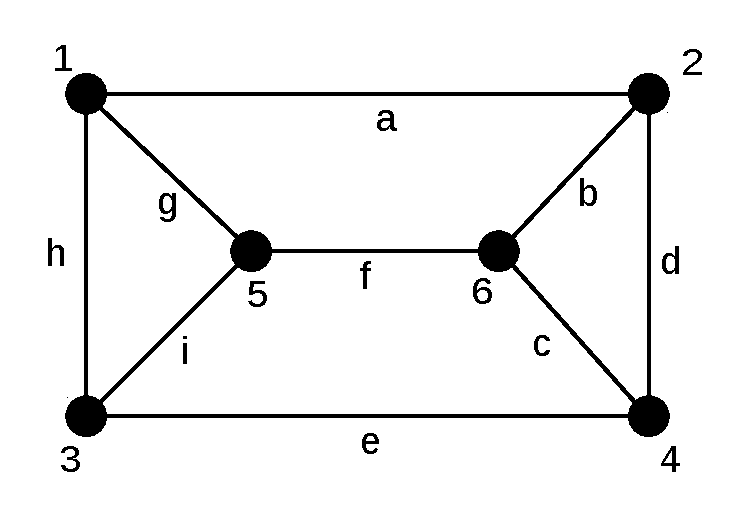
\includegraphics[scale=0.6]{graphExample.pdf}
	%\caption{Graph}
\end{figure}

\end{frame}

\begin{frame}
\frametitle{Graph Theory}
\begin{itemize}
	\item<1> A \textit{path} is a sequence of connected vertices and edges with no repeated vertices
	\item<2> A \textit{cycle} is a path except that the first vertex is the same as the last vertex
	\begin{figure}
	\centering
	\includegraphics<1>[scale=0.6]{pathExample.pdf}
	\includegraphics<2>[scale=0.6]{cycleExample.pdf}
	%\caption{Graph}
	\end{figure}
\end{itemize}
\end{frame}

\begin{frame}
\frametitle{Computational Complexity}
\begin{itemize}
	\item A decision problem returns a `yes' or `no' answer. 
	\item Polynomial time algorithms increase in steps by a factor of $n^k$ as input size $n$ increases. 
	\item Decision problems that can be verified by a polynomial time algorithm are in the class NP. 
	\item Verifying is not solving! 
	\begin{itemize}
		\item "Given a bag of 1000 keys and a door, is there a key in the bag that unlocks the door?"
		\item "Given one key, does it unlock the  door?"
	\end{itemize}
	\item Problems that are NP-hard are at least as hard as every problem in NP. 
\end{itemize}


\end{frame}

\begin{frame}
\frametitle{The Generalized Traveling Salesman Problem}
%\begin{columns}
%\begin{column}{0.5\textwidth}
\begin{itemize}
	\item The traveling salesman problem (TSP) is an NP-hard problem. 
	\begin{itemize}
		\item The goal is to find the minimum-cost cycle with all vertices. 
	\end{itemize}	
	\item The generalized traveling salesman problem (GTSP) is a generalization of the TSP. 
	\begin{itemize}
		\item Vertices are divided into disjoint subsets.
		\item The goal is to find the shortest cycle that contains one vertex from each subset.
	\end{itemize}
\end{itemize}
%\end{column}
%\begin{column}{0.5\textwidth}

%\end{column}
%\end{columns}
\end{frame}

%\begin{frame}
%\frametitle{IFD wins either way}

%\begin{columns}
%\begin{column}{0.6\textwidth}

%\begin{itemize}
%	\item IFD generates low-error individuals from tables evolved with IFD \textbf{and without IFD}.
%	\linespace
%	\item IFD's local search is valuable in all phases of the process, even if it wasn't used previously.
%	\linespace
%	\item N-gram GP isn't able to work effectively with the more complex probability tables that IFD generates.
%\end{itemize}
%\end{column}

%\begin{column}{0.02\textwidth}
%\end{column}

%\begin{column}{0.5\textwidth}

%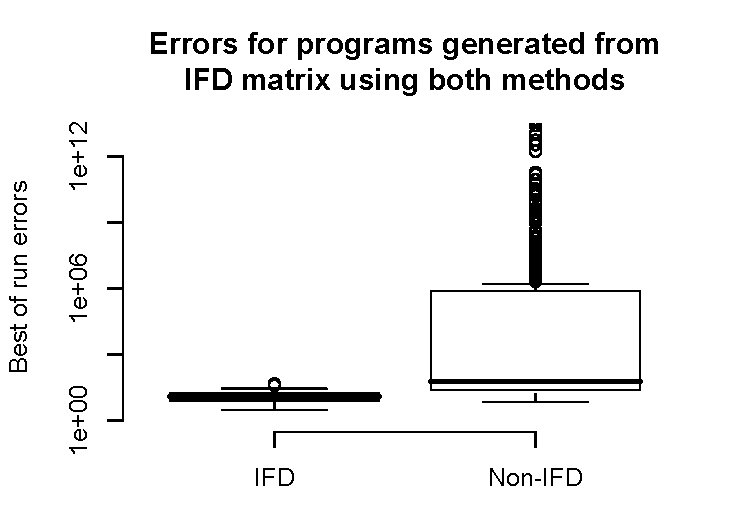
\includegraphics[width=0.915\textwidth]{ErrorsGenedProgsFromIfdMatrix.pdf}

%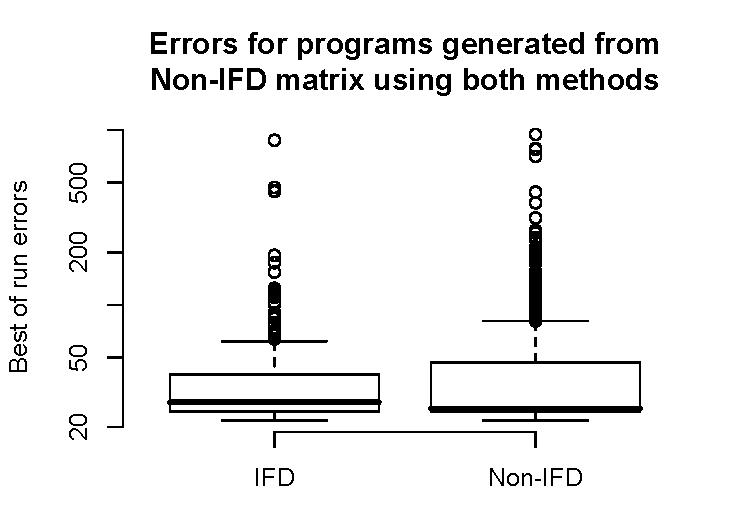
\includegraphics[width=0.915\textwidth]{ErrorsGenedProgsFromNonIfdMatrix.pdf}

%\end{column}
%\end{columns}

%\end{frame}

\section[Local-Global Search and Consultant Guided Search]{Local-Global Search and Consultant Guided Search}
\begin{frame}
	\frametitle{Local-Global Search}
\begin{itemize}
	\item Pop and Iordache
	\item A sequence $(V_{k_{1}}, V_{k_{2}}, ..., V_{k_{n}})$ of vertex subsets is chosen.
	\item Subset $V_{k_{1}}$ is duplicated and added to the end of the sequence.
	\item Shortest path that contains vertices from all subsets is found. 
	\item Local-global search does not lead to an optimal solution. 
\end{itemize}
\begin{figure}
	\centering
	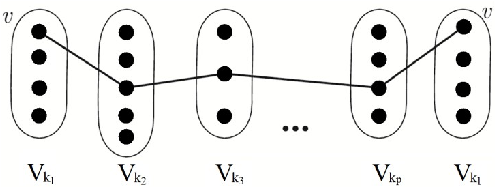
\includegraphics[scale=0.9]{LocalGlobalExampleRevised.pdf}
	\caption{Adapted from Pop and Iordache}
\end{figure}

\end{frame}

\begin{frame}
\frametitle{Local-Global Search}
\begin{center}
$(V_{1},V_{2},V_{3},V_{4},V_{1})$
\end{center}
\begin{figure}
	\centering
	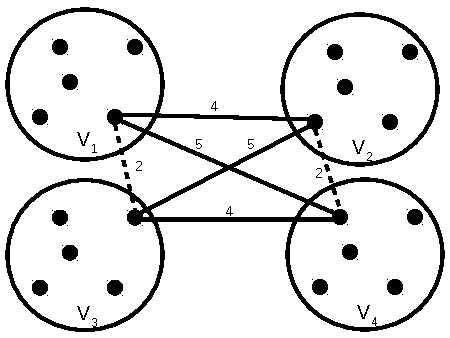
\includegraphics{localglobal2revised.pdf}
\end{figure}

\end{frame}

\begin{frame}
\frametitle{Consultant Guided Search}
	\begin{itemize}
	\item Swarm Intelligence
	\item Simulated individuals each take on roles of ``consultant'' and ``client.''
	\item Each virtual client chooses a consultant based on consultants' ``reputation.''
	\item The consultant gives the client suggestions.
	\item The client may or may not take the consultant's suggestion. 
	\item The consultant's reputation changes based on the performance of the clients. 
	\end{itemize}

\end{frame}

\begin{frame}
\frametitle{The Hybrid Algorithm}
\begin{itemize}
	\item The consultant constructs a cycle of vertex subsets. 
	\item The client builds a sequence of vertex subsets. 
	\item The consultant suggests the next vertex subset. 
	\item After a sequence is found, local-global search is used to find the best cycle given the sequence. 
	\item Variant: Each edge has a confidence value. 
\end{itemize}
\begin{figure}
	\centering
	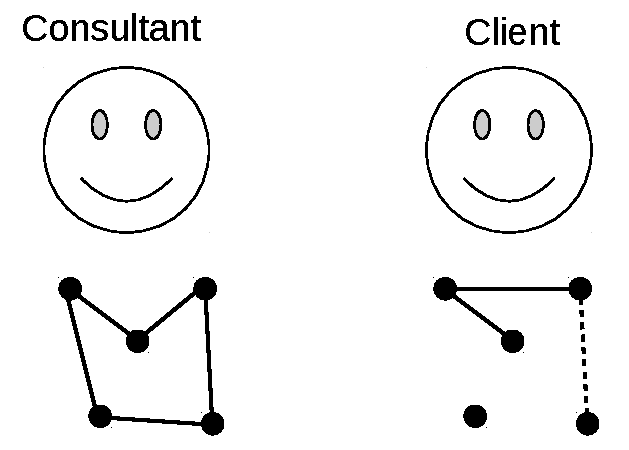
\includegraphics[scale=0.55]{CGSExample.pdf}

\end{figure}

\end{frame}

\begin{frame}
\frametitle{Results}
\begin{itemize}
	\item Regular algorithm and variant were compared to the best known algorithm at the time. 
	\item Variant was statistically similar to the best known algorithm. 
	\item Variant was much better in some cases. 
\end{itemize}
\end{frame}


\section[Variable Neighborhood Search]{Variable Neighborhood Search}

\begin{frame}
\frametitle{Cluster-Based Local Search}
	\begin{itemize}
	\item CBLS starts with a sequence, finds best vertices within each vertex subset (or \textit{cluster}).
	\item The sequence is changed after every iteration. 
	\item The algorithm returns the best cycle after certain permutations are tried. 
	\end{itemize}
\begin{figure}
	\centering
	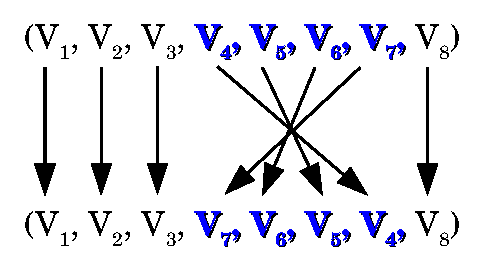
\includegraphics[scale=0.8]{CBLSExample.pdf}
\end{figure}

\end{frame}

\begin{frame}
\frametitle{Node-Based Local Search}
	\begin{itemize}
	\item Starts with a vertex chosen in each subset, then finds the best sequence of vertices. 
	\item Exact or approximate algorithms can be used to find the sequence of vertices. 
	\item The vertices chosen are changed after every iteration.
	\item The algorithm returns the best cycle and vertices after certain vertices are tried. 
	\end{itemize}
\begin{figure}
	\centering
	\includegraphics<1>[scale=0.4]{NBLSExample1.pdf}
	\includegraphics<2>[scale=0.4]{NBLSExample2.pdf}
\end{figure}
\end{frame}

\begin{frame}
\frametitle{Variable Neighborhood Search}
\begin{itemize}
	\item VNS combines the two search algorithms. 
	\item Cluster-based local search is used first.
	\item Once CBLS has found a local optimum, node-based local search is used. 
\end{itemize}
\end{frame}

\begin{frame}
	\frametitle{Advantages and Disadvantages}
	\begin{itemize}	
		\item Cluster-based local search and node-based local search could each be used alone. 
		\item Which method is best in what situations? 
		\item Why use variable-neighborhood search?
		\item Pourhassan and Neumann, University of Adelaide, Australia
	\end{itemize}
\end{frame}

\begin{frame}
\frametitle{Advantages of Node-Based Local Search}
\begin{figure}
	\centering
	\includegraphics<1>{GTSPCase1.pdf}
	\includegraphics<2>{Instance1Colored2.pdf}
	\includegraphics<3>{Instance1Colored1.pdf}
	\caption{An instance that is hard for Cluster-Based Local Search (Taken from Pourhassan and Neumann)}
\end{figure}
\end{frame}

\begin{frame}
\frametitle{Advantages of Cluster-Based Local Search}
\begin{figure}
	\centering
	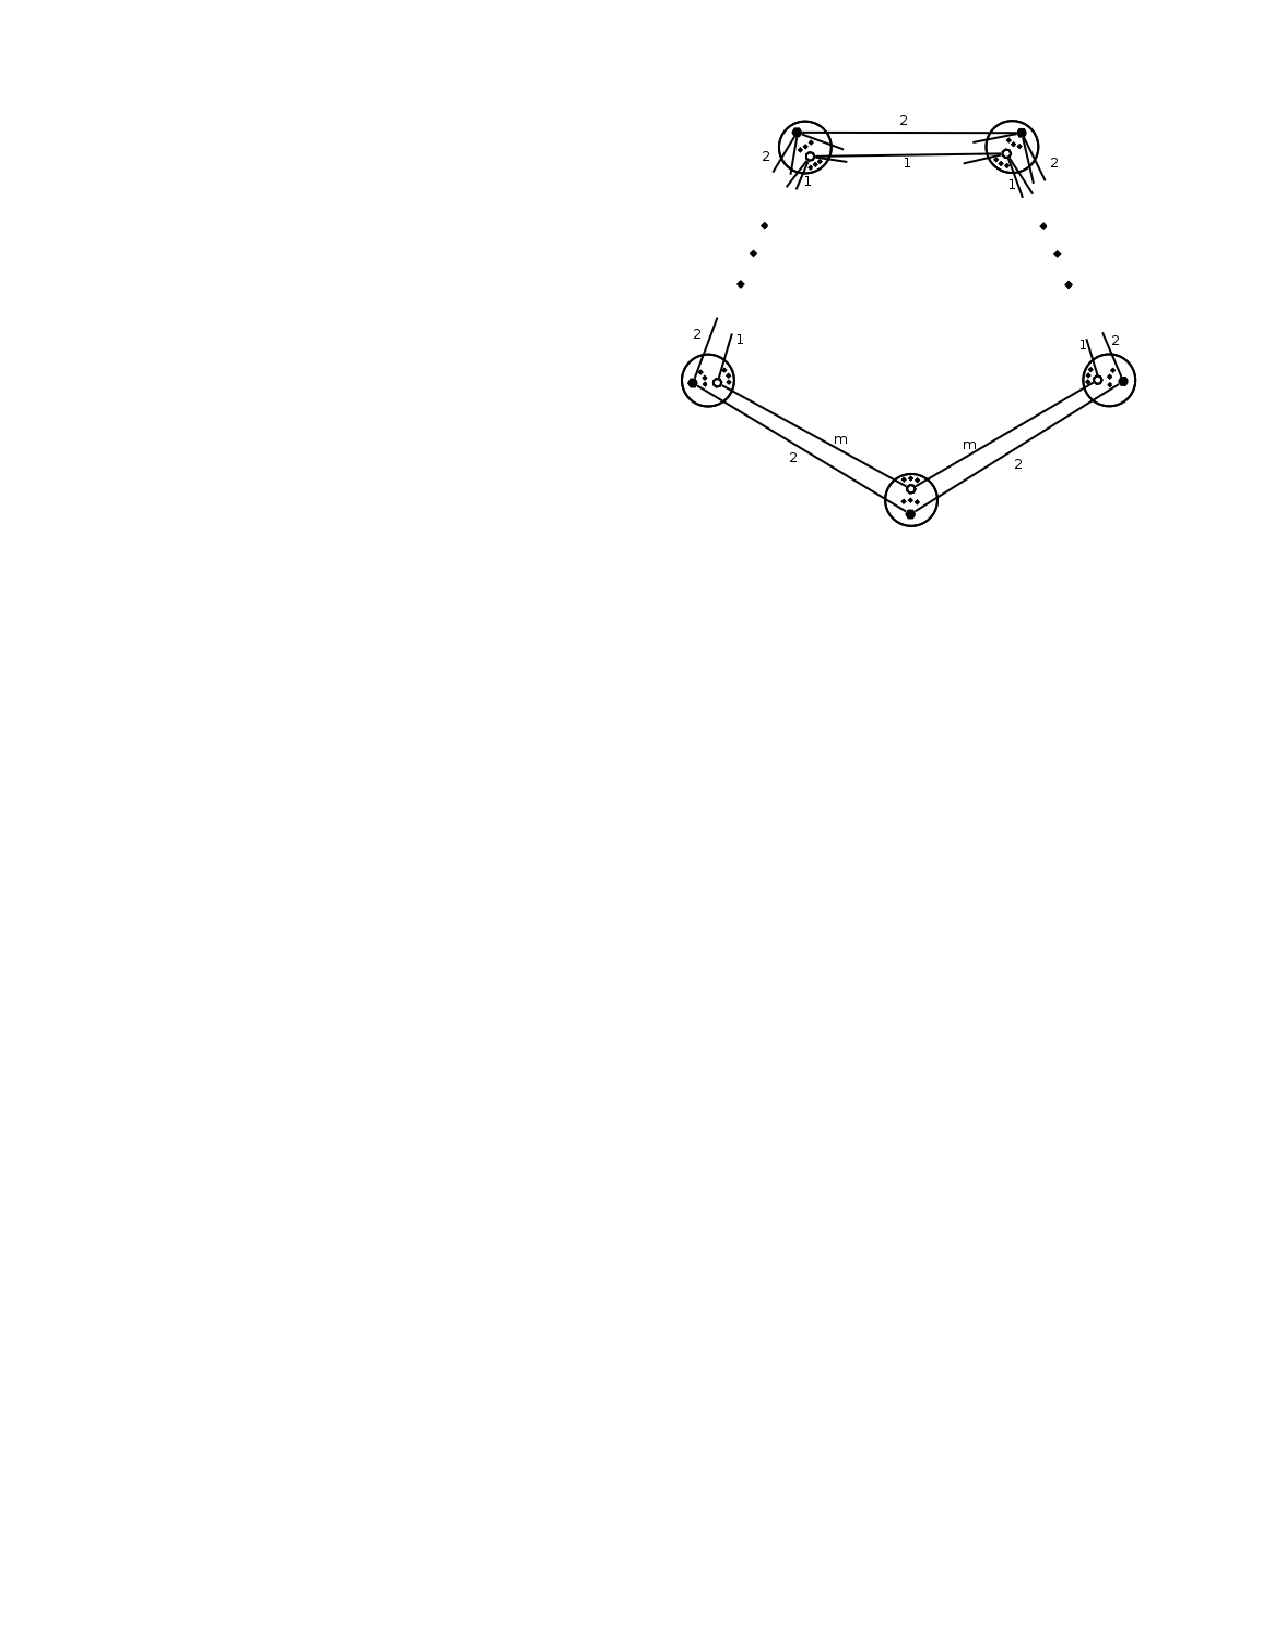
\includegraphics[scale=0.8]{GTSPCase2.pdf}
	\caption{An instance that is hard for Node-Based Local Search, where m is the total number of subsets (Taken from Pourhassan and Neumann)}
\end{figure}
\end{frame}

\begin{frame}
\frametitle{Advantages of Variable Neighborhood Search}
\begin{figure}
	\centering
	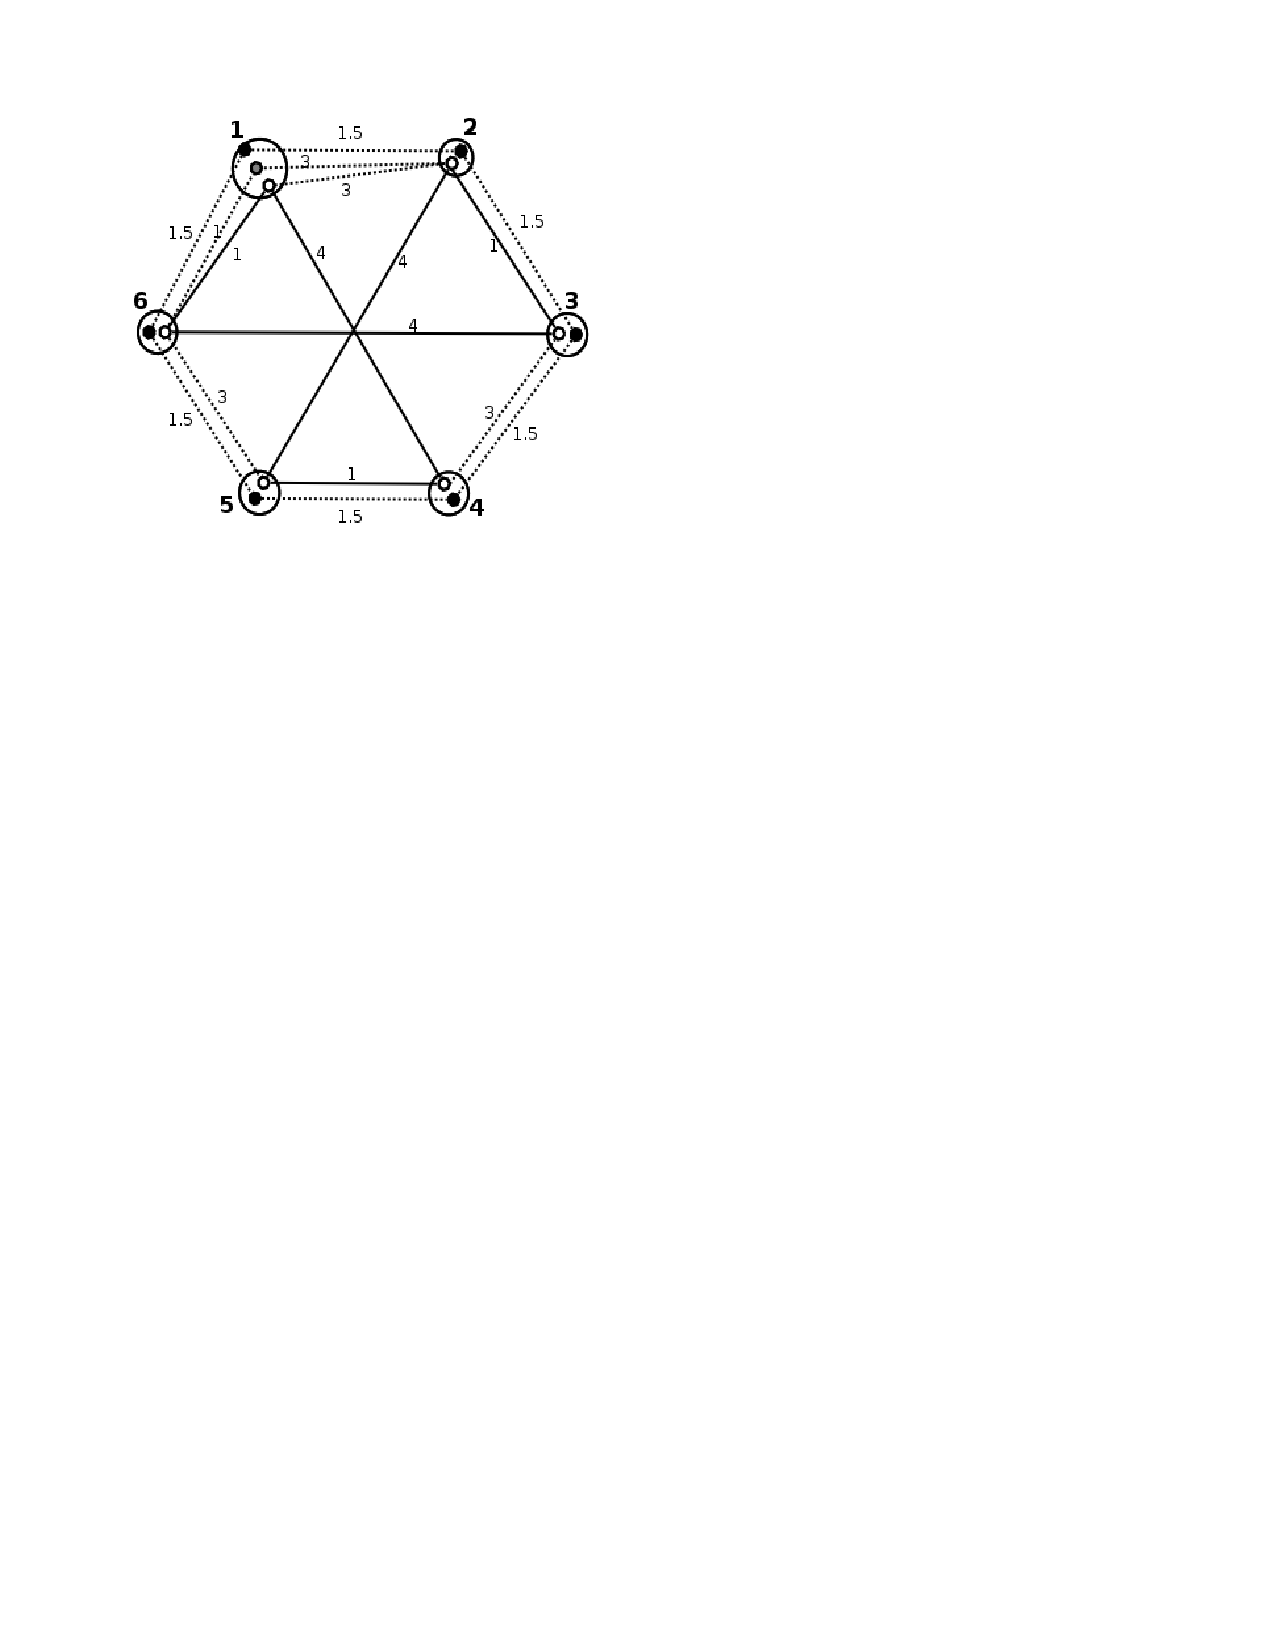
\includegraphics[scale=0.8]{GTSPCase3.pdf}
	\caption{An instance that is hard for either but easy with VNS (taken from Pourhassan and Neumann)}
\end{figure}
\end{frame}

\section[Conclusions]{Conclusions}

\begin{frame}
	\frametitle{Conclusions}
	\begin{itemize}
	\item The GTSP is computationally intensive.
	\item Heuristics are effective for many practical purposes.
	\item Different heuristics have different strengths.
	\item Combining heuristics can increase effectiveness.
	\end{itemize}	
\end{frame}

%\begin{frame}
%\end{frame}



\section*{References}

\begin{frame} 
	\frametitle{References} 
	\begin{thebibliography}{lskdjf}
	\bibitem{Pop:2011}
P.C. Pop and S. Iordache.
A hybrid heuristic approach for solving the generalized traveling salesman problem.
\newblock In \textit{Proceedings of the 13th Annual Conference on Genetic and Evolutionary Computation}, GECCO '11, pages 481-488, New York, NY, USA, 2011. ACM. 
	
	\bibitem{Pourhassan:2015}
M. Pourhassan and F. Neumann.
On the impact of local search operators and variable neighbourhood search for the generalized travelling salesperson problem.
\newblock In \textit{Proceedings of the 2015 Annual Conference on Genetic and Evolutionary Computation}, GECCO '15, pages 465-472, New York, NY, USA, 2015. ACM. 
  
  	\end{thebibliography}
	\linespace

\end{frame} 
\section*{Questions?}
\begin{frame}
\frametitle{Thank you!}
\begin{center}
\begin{large}
	Questions?
\end{large}
\end{center}
\end{frame}

\end{document}


